\documentclass[border=10pt]{standalone}
\usepackage{pgfplots}
\pgfplotsset{compat=1.18}

\begin{document}
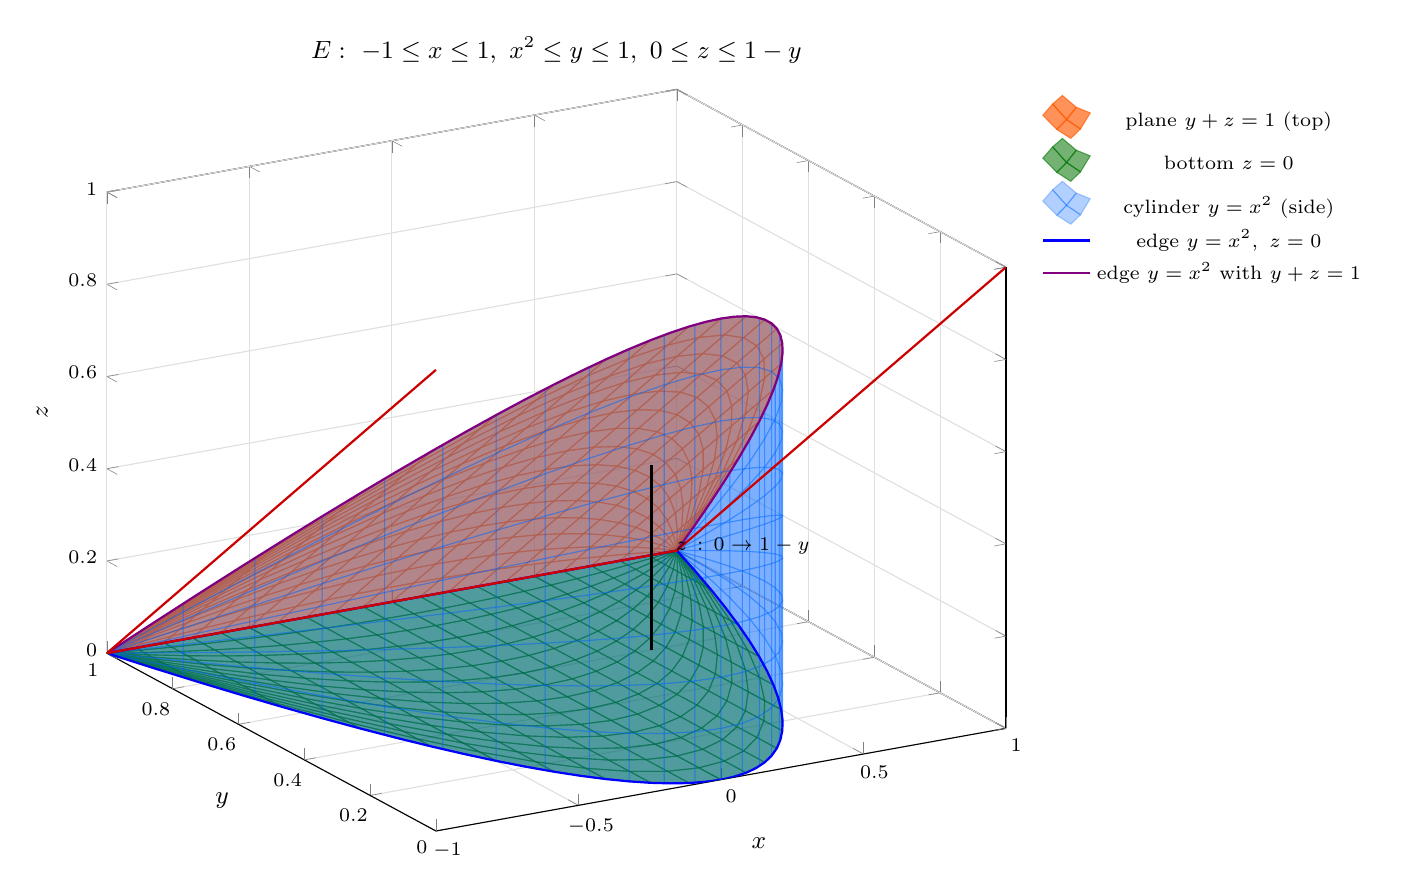
\begin{tikzpicture}
\begin{axis}[
    width=13cm, height=11cm,
    view={-30}{24},
    xmin=-1,xmax=1, ymin=0,ymax=1, zmin=0,zmax=1,
    xlabel=$x$, ylabel=$y$, zlabel=$z$,
    tick label style={font=\scriptsize}, label style={font=\small},
    title={$E:\ -1\le x\le 1,\ x^2\le y\le 1,\ 0\le z\le 1-y$},
    title style={font=\small},
    legend pos=outer north east, legend style={font=\scriptsize, draw=none},
    grid=major, grid style={gray!25},
]
% slanted plane z = 1-y (top lid)
\addplot3[surf, color=orange!70!red, opacity=0.65, shader=flat,
          domain=-1:1, samples=21, domain y=0:1, samples y=16]
    ({x}, {x^2 + y*(1-x^2)}, {1-(x^2 + y*(1-x^2))});
\addlegendentry{plane $y+z=1$ (top)}

% bottom z = 0
\addplot3[surf, color=green!45!black, opacity=0.55, shader=flat,
          domain=-1:1, samples=21, domain y=0:1, samples y=16]
    ({x}, {x^2 + y*(1-x^2)}, {0});
\addlegendentry{bottom $z=0$}

% parabolic cylinder y = x^2 (curved side wall)
\addplot3[surf, color=blue!60!cyan, opacity=0.30, shader=flat,
          domain=-1:1, samples=25, domain y=0:1, samples y=10]
    ({x}, {x^2}, {(1-x^2)*y});
\addlegendentry{cylinder $y=x^2$ (side)}

\addplot3[thick, blue, domain=-1:1, samples=41] ({x},{x^2},{0});
\addlegendentry{edge $y=x^2,\ z=0$}
\addplot3[thick, violet, domain=-1:1, samples=41] ({x},{x^2},{1-x^2});
\addlegendentry{edge $y=x^2$ with $y+z=1$}
\addplot3[thick, red!80!black, domain=0:1, samples=11] ({1},{x},{1-x});
\addplot3[thick, red!80!black, domain=0:1, samples=11] ({-1},{x},{1-x});
\addplot3[thick, red!80!black, domain=-1:1, samples=11] ({x},{1},{0});
\addplot3[very thick, black, domain=0:0.4, samples=11] ({0.45},{0.6},{x});
\node[font=\scriptsize, anchor=west] at (axis cs:0.5,0.6,0.22) {$z\,:\,0\to 1-y$};
\end{axis}
\end{tikzpicture}
\end{document}
